% this TeX file provides an awesome example of how TeX will make super 
% awesome tables, at the cost of your of what happens when you try to make a
% table that is very complicated.
\documentclass[11pt]{article}

% Use wide margins, but not quite so wide as fullpage.sty
\marginparwidth 0.5in 
\oddsidemargin 0.25in 
\evensidemargin 0.25in 
\marginparsep 0.25in
\topmargin 0.25in
\textwidth 6in
\textheight 8in
% That's about enough definitions

% language input
\usepackage[utf8]{inputenc}
% multirow allows you to combine rows in columns
\usepackage{multirow}
% tabularx allows manual tweaking of column width
\usepackage{tabularx}
% insert images
\usepackage{graphicx}
\usepackage{float}
\graphicspath{ {images/} }

\begin{document}
% this is an alternate method of creating a title
%\hfill\vbox{\hbox{Gius, Mark}
%       \hbox{Cpe 456, Section 01}  
%       \hbox{Lab 1}    
%       \hbox{\today}}\par
%
%\bigskip
%\bigskip
\author{Vandré Leal Cândido}
\title{Wireshark Lab: IP v6.0}
\maketitle

% 2. A look at the captured trace
\section{A look at the captured trace}

\begin{itemize}
	\setlength\itemsep{.5cm}

	\item
		\textit{Select the first ICMP Echo Request message sent by your computer, and expand the Internet Protocol part of the packet in the packet details window. What is the IP address of your computer?}
		\par The IP address of my computer is 192.168.0.1.
		
		\begin{figure}[H]
		\centering
		\caption{Local IP address}
		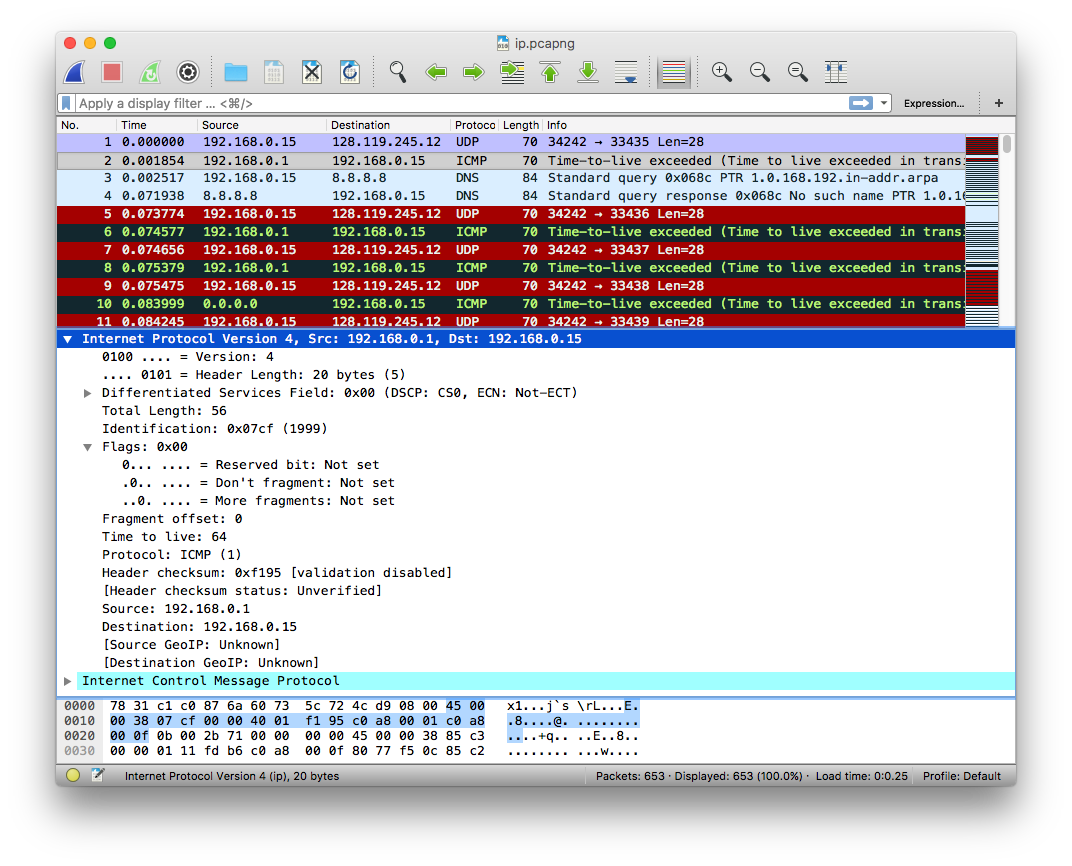
\includegraphics[width=400px]{01}
		\end{figure}
		
		\par The previous screenshot is also used to answer the following questions.

	\item
		\textit{Within the IP packet header, what is the value in the upper layer protocol field?}
		\par The value in the upper layer protocol field is ICMP (1).

	\item
		\textit{How many bytes are in the IP header? How many bytes are in the payload of the IP
datagram? Explain how you determined the number of payload bytes.}
		\par There are 20 bytes in the header. The payload is 36 bytes since it is the length of the datagram subtracted by the number of header bytes  (56 - 20 = 36).
		
	\item
		\textit{Has this IP datagram been fragmented? Explain how you determined whether or not the
datagram has been fragmented.}
		\par This datagram hasn't been fragmented since the \textbf{More fragments} flag is not set.
		
	\item
		\textit{Which fields in the IP datagram always change from one datagram to the next within this series of ICMP messages sent by your computer?}
		\par Three fields always change from one ICMP message to another: \textbf{Identification}, \textbf{Time to live} and \textbf{Header checksum}.
		
	\item
		\textit{Which fields stay constant? Which of the fields must stay constant? Which fields must change? Why?}
		\par The following fields stay constant and must stay constant:
		\begin{itemize}
			\item Version: IPv4.
			\item Header length: constant value (20 bytes) for all ICMP packets.
			\item Source: sending from the same source.
			\item Destination: sending to the same destination.
			\item Differentiated Services: all ICMP packets use the same service class.
			\item Upper Layer Protocol: IMCP(1) for all ICMP packets.
		\end{itemize}
		
		\par The fields that must change are the ones mentioned in the previous question:
		\begin{itemize}
			\item Identification: IP packets must have different identification numbers.
			\item Time to live: traceroute increments the value.
			\item Header checksum: since the header changes the checksum must change as well.
		\end{itemize}
		
	\item
		\textit{Describe the pattern you see in the values in the Identification field of the IP datagram.}
		\par The Identification field value is incremented on every new ICMP message.
		
	\item
		\textit{What is the value in the Identification field and the TTL field?}
		\par Identification: 0x07cf (1999).
		\newline TTL: 64.
		
	\item
		\textit{Do these values remain unchanged for all of the ICMP TTL-exceeded replies sent to your
computer by the nearest (first hop) router? Why?}
		\par The Identification field value changes for all of the ICMP TTL-exceeded replies since it's an unique value. Two or more datagrams only have the same identification value in case they are fragments of a single large datagram. The TTL value remains unchanged because the TTL for the first router has always the same value.
	
\end{itemize}

% 3. Fragmentation
\section{Fragmentation}

\begin{itemize}
	\setlength\itemsep{.5cm}

	\item
		\textit{Find the first ICMP Echo Request message that was sent by your computer after you
changed the Packet Size in pingplotter to be 2000. Has that message been fragmented across
more than one IP datagram? [Note: if you find your packet has not been fragmented, you
should download the zip file http://gaia.cs.umass.edu/wireshark-labs/wireshark-traces.zip and
 extract the ipethereal-trace-1packet trace. If your computer has an Ethernet interface, a packet 3
size of 2000 should cause fragmentation.]}
		\par The file suggested was downloaded and will be used in this section since the message hasn't been fragmented on my tests.

\pagebreak

	\item
		\textit{Print out the first fragment of the fragmented IP datagram. What information in the IP header indicates that the datagram been fragmented? What information in the IP header indicates whether this is the first fragment versus a latter fragment? How long is this IP datagram?}
		\par The flag \textbf{More fragments} set to 1 indicates that the datagram has been fragmented. The field \textbf{Fragment offset} set to 0 indicates that this is the first fragment, otherwise the value of this field would be greater than 0. The datagram has a total length of 1500 bytes, including the header.
		
		\begin{figure}[H]
		\centering
		\caption{First datagram (packet size=2000)}
		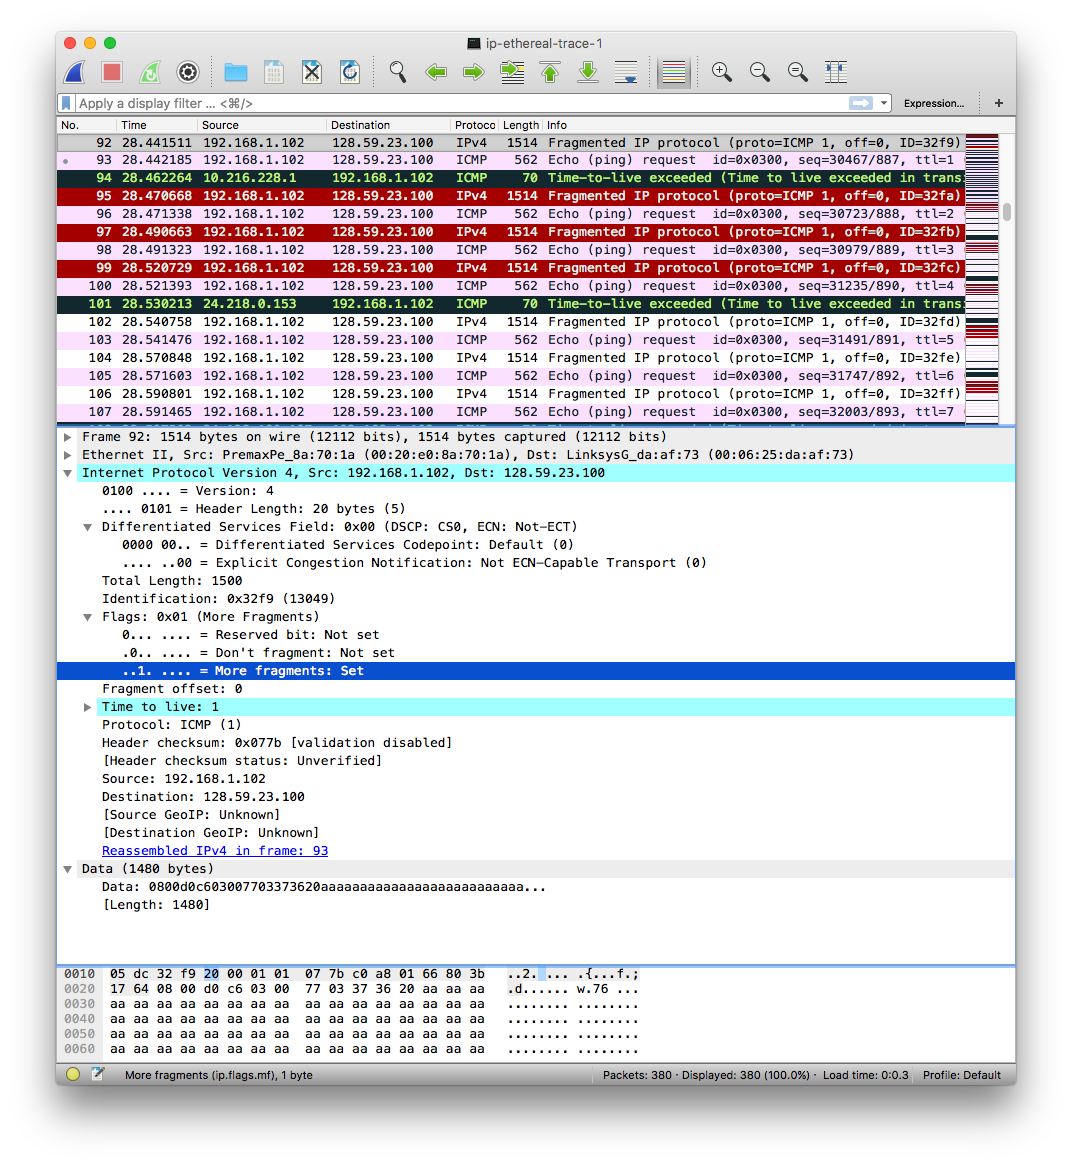
\includegraphics[width=380px]{02}
		\end{figure}
		
	\item
		\textit{Print out the second fragment of the fragmented IP datagram. What information in the IP header indicates that this is not the first datagram fragment? Are the more fragments? How can you tell?}
		\par The value of the field \textbf{Fragment offset} is 1480 and indicates that this is the second and last fragment since the flag \textbf{More fragments} is not set.
		
		\begin{figure}[H]
		\centering
		\caption{Second datagram (packet size=2000)}
		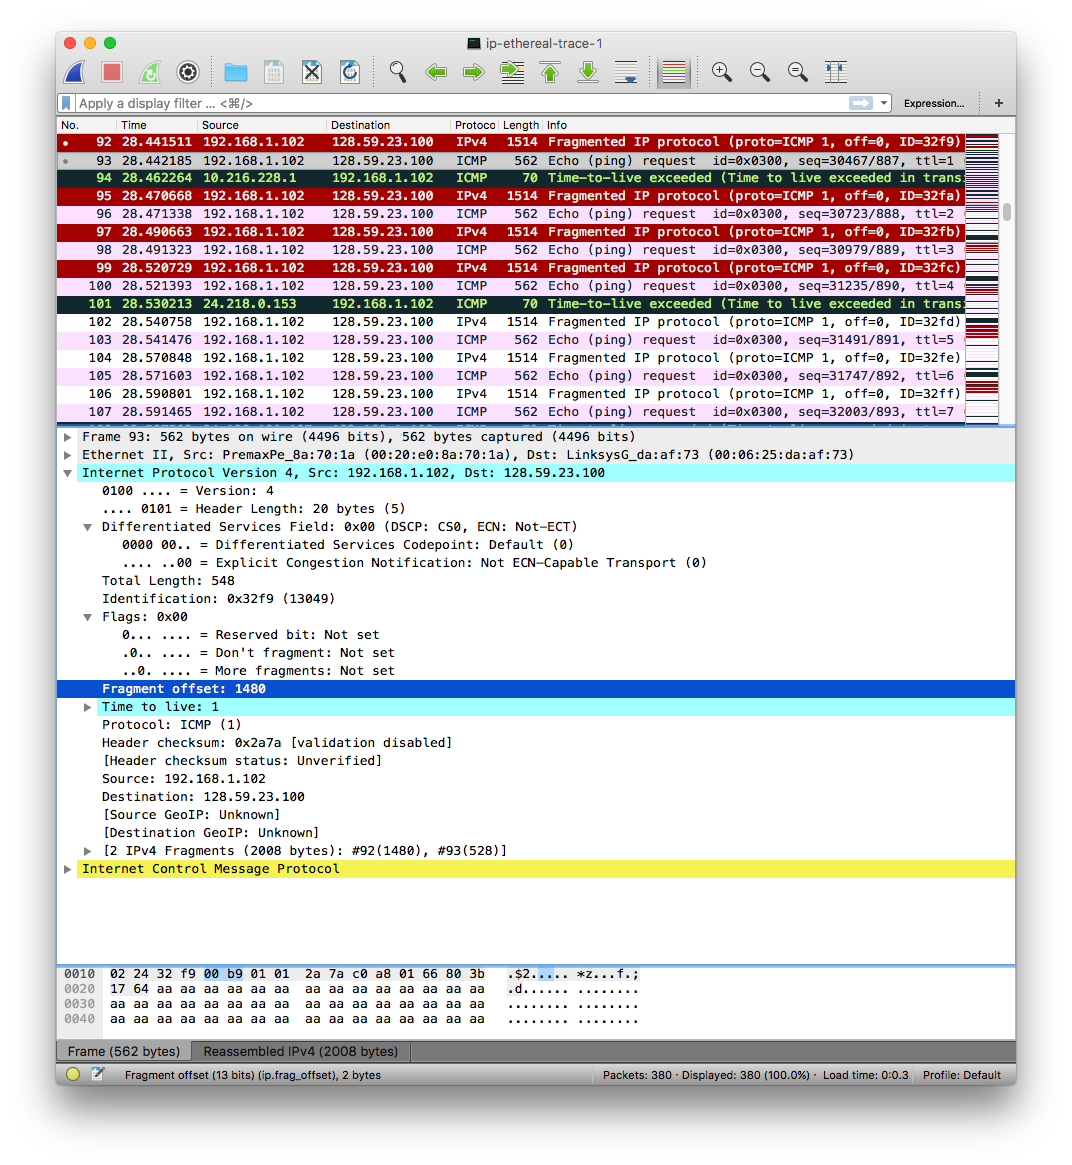
\includegraphics[width=380px]{03}
		\end{figure}
		
\pagebreak

\par Now find the first ICMP Echo Request message that was sent by your computer after you changed the
Packet Size in pingplotter to be 3500.

	\item
		\textit{What fields change in the IP header between the first and second fragment?}
		\par The fields that changed between the first and second fragment are: \textbf{Total Length}, \textbf{Flags}, \textbf{Fragment offset} and \textbf{Header checksum}
		
	\item
		\textit{How many fragments were created from the original datagram?}
		\par Three fragments were created after switching the packet size to 3500.
		
	\item
		\textit{What fields change in the IP header among the fragments?}
		\par The fields that changed between all the fragments are: \textbf{Fragment offset} and \textbf{Header checksum}. \textbf{Total Length} and \textbf{Flags} are only changed between the first two packets and the last one since both the first and the second fragments have a total length of 1500 with the flag \textbf{More fragments} set to 1, whereas the last packet has a total length of 540 with the flag \textbf{More fragments} not set.
		
		\begin{figure}[H]
		\centering
		\caption{First datagram (packet size=3500)}
		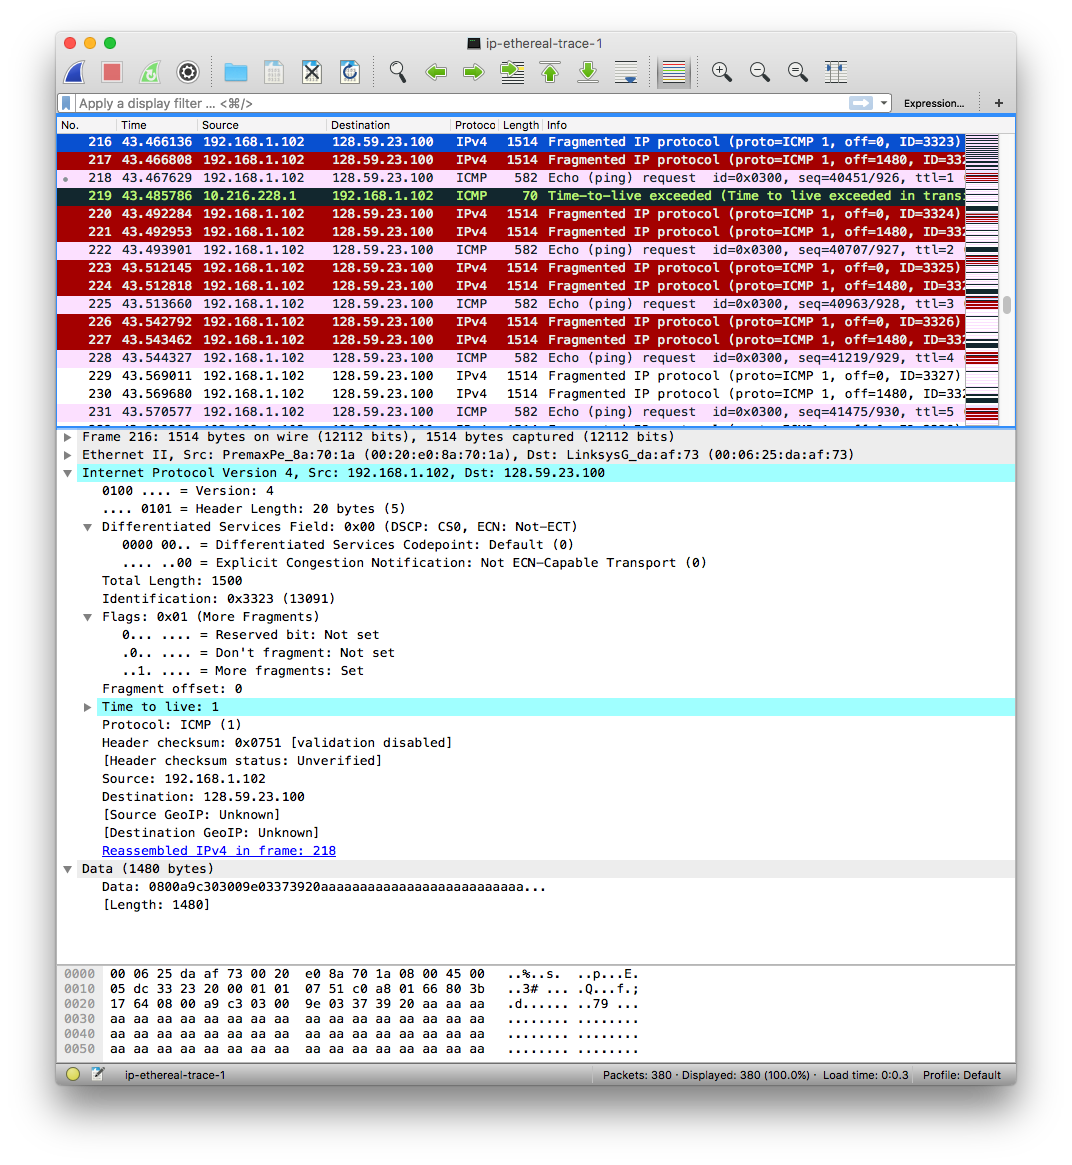
\includegraphics[width=\textwidth]{04}
		\end{figure}
		
		\begin{figure}[H]
		\centering
		\caption{Second datagram (packet size=3500)}
		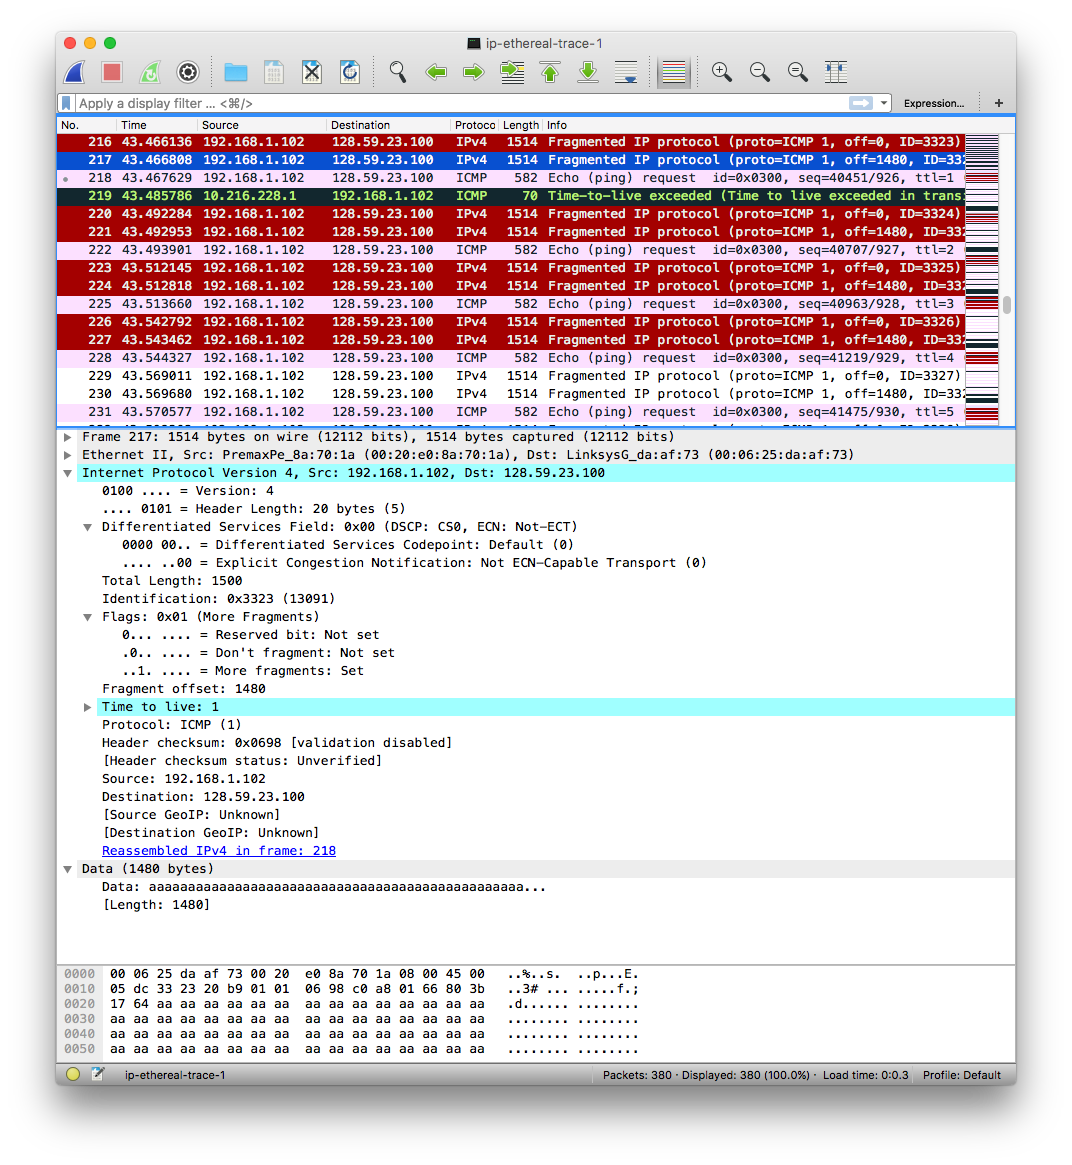
\includegraphics[width=\textwidth]{05}
		\end{figure}
		
		\begin{figure}[H]
		\centering
		\caption{Third datagram (packet size=3500)}
		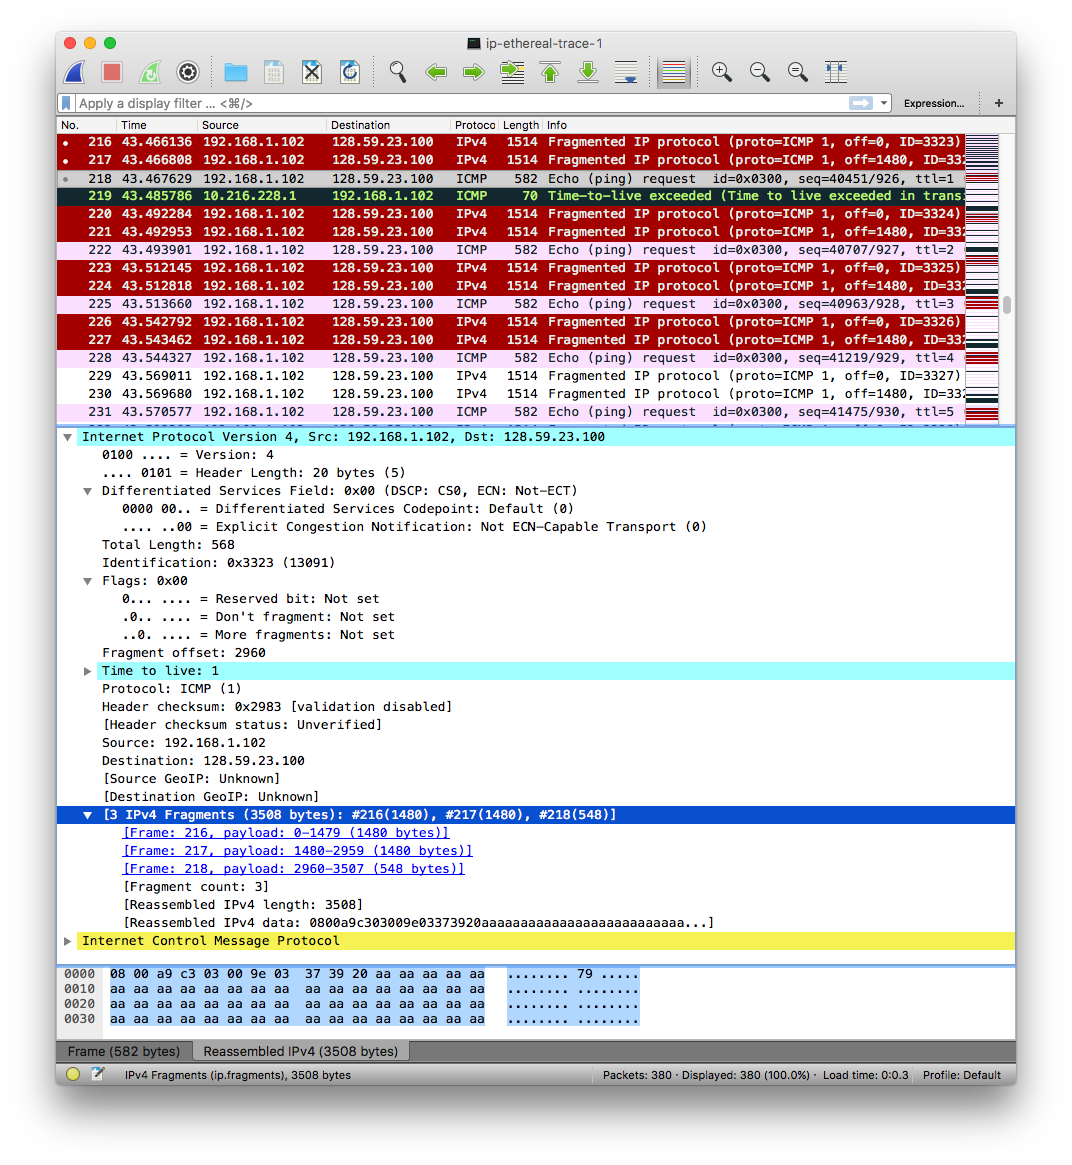
\includegraphics[width=\textwidth]{06}
		\end{figure}

\end{itemize}

\end{document}
